\cotefile{101}
\scanpage{2}
\uline{Relations entre} \uline{cohomologie locale} et \uline{projective} (via \uline{les} \uline{cônes})
% archive sheet number: 1

\scanpage{3}
\uline{Relations entre cohomologie locale et globale}

$Y$ préschéma de base

$\underline S$ Algèbre graduée \unsure{quasi cohérente|qu. cohérente|quasi-cohérente}, à degrés $\geq 0$, engendrée par $\underline S_1$ de type fini
\[
 X=\operatorname{Proj}(S)
\]
\[
 X'=\operatorname{Spec}(S)-Y \qquad \text{cône épointé},\quad
 \overline{X'}\ \deleted{\unsure{C|=|\text{le}}}\ \text{cône affine}
\]
\[
 X'\simeq\mathrm V(\underline O_X(-1))-o(X)
 =\operatorname{Spec}\,\deleted{\unsure{\underline{\operatorname{Sym}}(\,|{\operatorname{Sym}}(\,}}%
 \coprod_{n\in\mathbb Z}\underline O(-n)
\]

Soit $Z$ une partie fermée de $X$, $Z'$ son image inverse dans $X'$, $\overline{Z'}$ son adhérence [défini aussi au dessus de l'Idéal homogène définissant $Z$].

$U$ ouvert de $X$, $U'$ image inverse dans $X'$, $\overline{U'}$ ds $\overline{X'}$.

Soient $F,G$ deux Modules [qu. coh.] sur $U$, $F',G'$ leurs images inverses sur $U'$. \deleted{\unsure{On aura}}
\[
\begin{aligned}
 \operatorname{Ext}^{\bullet}_{\underbrace{Z'\cap U'}_{T'}}(X';F',G')
 &=H^{\bullet}\deleted{\unsure{\Gamma_{Z'\cap U'}}}
 \operatorname{Hom}_{\underbrace{Z'\cap U'}_{T'}}(F',\unsure{\mathrm{Cl}|\mathrm C\ell|\mathrm C(}G')\\
 &=H^{\bullet}\deleted{\unsure{\Gamma_{Z\cap U}\,p_U}}
 \operatorname{Hom}_{\underbrace{Z\cap U}_{T}}(F,p_U\mathrm{Cl}G')\\
 &=H^{\bullet}\operatorname{Hom}_{\underbrace{Z\cap U}_{T}}(F,\mathrm{Cl}\,p_U G')\\
 &=\unsure{\mathbb E|E}\mathrm{xt}^{\bullet}_{\underbrace{Z\cap U}_{T}}
 (F,\coprod_{n\in\mathbb Z}G(n))
\end{aligned}
\]
\margin{$T=U\cap Z$ loc fermé \inserted{dans $X$}\\ $T'=U'\cap Z'$}
\margin{$\left\{\vphantom{\dfrac{G}{G}}\right.$ $G$ qu. coh.}
\margin{$\left\}\vphantom{\dfrac{F}{F}}\right.$ $F\left|\begin{array}{l}\text{qu. coh}\\\text{type fini}\end{array}\right.$}
\[
 \boxed{{\unsure{\operatorname{Ext}|\operatorname{Idt}}}^{\bullet}_{\deleted{\unsure{Z'}}T'\!,\,\underline O_{X'}}(X';F',G')
 =\coprod_{n\in\mathbb Z}\operatorname{Ext}^{\bullet}_{T\deleted{\unsure{,\,\underline O}}}(F,G(n))}
\]
\margin{$p:X'\longrightarrow X$\\ $p_U:U'\longrightarrow U$}
% archive sheet number: 2

\scanpage{4}
Localisant sur $Y$, on trouve
\[
 \underline{\operatorname{Ext}}^{\bullet}_{T'\deleted{\unsure{,Z'}},\,\unsure{\underline O_{U'}|\underline O_{X'}|\underline O_{\overline{X'}}}}
 (\overline{X'}/Y;\overline{F'},\overline{G'})
 \simeq\coprod_{n\in\mathbb Z}\underline{\operatorname{Ext}}^{\bullet}_{T\deleted{\unsure{\cap U}},\,\underline O_U}(X/Y;F,G(n))
\]
% slanted
\margin{N.B. \unsure{partir} \unsure{de modules|des modules} gradués,\ldots}
\[
 \deleted{\underline{\operatorname{Ext}}_{Z'\cap U'}}
\]
\deleted{D'autre part, on aura supposant pour simplifier $U=X$, donc $U'=X'$, $\overline{U'}=\overline{X'}$}
\[
 \deleted{\operatorname{Ext}^{\bullet}_{Z'\unsure{\cap U'},\,\underline O_{X'}}(X';F',G')
 \Longleftarrow H^p_{Z'}(X',\underline{\operatorname{Ext}}^q(F',G'\unsure{)\,)|\,}))}
\]
\figure{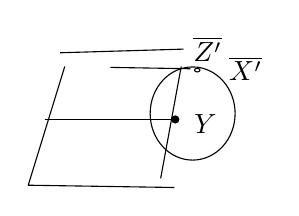
\begin{tikzpicture}[x=.58cm,y=.58cm]
 \draw (0,0)--(3.2,-.05) (0,0)--(.8,2.6) (2.9,.15)--(3.35,2.6);
 \draw (.7,2.9)--(3.4,2.98) node[right] {$\overline{Z'}$};
 \draw (1.8,2.58)--(3.55,2.55) (3.7,2.52) ellipse (.06 and .04);
 \draw (3.6,1.57) ellipse (.93 and 1.02);
 \draw (.36,1.44)--(3.22,1.44); \fill (3.22,1.44) circle (.09);
 \node at (3.88,1.35) {$Y$}; \node at (4.76,2.55) {$\overline{X'}$};
\end{tikzpicture}}
\figure{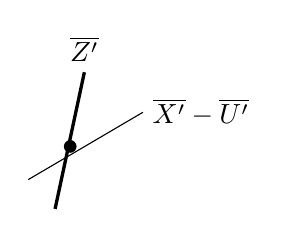
\begin{tikzpicture}[scale=.62]
 \draw[very thick] (.55,-1.3)--(1.15,1.5) node[above] {$\overline{Z'}$};
 \draw (0,-.7)--(2.35,.68) node[right] {$\overline{X'}-\overline{U'}$}; \fill (.86,-.02) circle (.13);
\end{tikzpicture}}
\diagram{\begin{tikzcd}[ampersand replacement=\&,row sep=small]
 \operatorname{Ext}^{\bullet}_{\overline{T'}\deleted{\unsure{,Z'}}}(\overline{X'};\overline{F'},\overline{G'})\\
 \operatorname{Ext}^{\bullet}_{\widehat{T'}}(\widehat{X'};\widehat{F'},\widehat{G'})\arrow[u]
\end{tikzcd}}
\figure{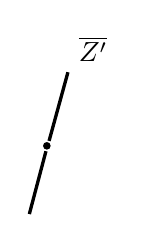
\begin{tikzpicture}[scale=.57]
 \draw[very thick] (.2,-1.5)--(.57,-.1) (.64,.13)--(1.06,1.66) node[above right] {$\overline{Z'}$}; \fill (.59,.02) circle (.085);
\end{tikzpicture}}
\[
 \underline H^p\bigl(\overline{Z'}\underset{\unsure{?}}{-}\overline{R'},
 \overbrace{\underline{\operatorname{Ext}}^{q}_{\overline{Z'}}(\overline{F'},\overline{G'})}\bigr)
\]
\margin{formation de ces \unsure{invariants} est compatible aux extensions plates de la base\ldots}
\figure{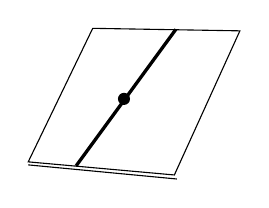
\begin{tikzpicture}[scale=.64]
 \draw (0,0)--(2.9,-.26)--(4.2,2.6)--(1.28,2.65)--cycle;
 \draw (0,-.06)--(2.95,-.34); \draw[very thick] (.95,-.08)--(2.93,2.63); \fill (1.9,1.25) circle (.12);
\end{tikzpicture}}
\[
 H^p(\overline{Z'}-\overline{R'},\overline E)
 \mathrel{\overset{\unsure{?|2}}{\underset{\longleftrightarrow}{\sim}}}
 H^p(\widehat{Z'}-\widehat{R'},\widehat E)
\]
\margin{\deleted{\unsure{par hypothèse|bij.-bij.}} \unsure{par localisé|pour localisé|par localis.}}
Le lemme des cinq nous ramène au cas des $H^p_{\overline{Z'}}(\overline{R'},\overline E)$, ou en changeant de \unsure{notations|notation} les $H^p_{\overline{Z'}}(\overline{X'},\overline E)$
\figure{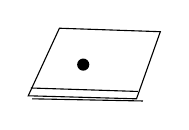
\begin{tikzpicture}[scale=.55]
 \draw (0,0)--(2.5,-.07)--(3.05,1.48)--(.72,1.56)--cycle;
 \draw (.06,.18)--(2.53,.1) (.09,-.07)--(2.65,-.12); \fill (1.27,.72) circle (.14);
\end{tikzpicture}}
\deleted{Mais ceci est} \unsure{Dégager|D'après|Dégageons} un \uline{lemme} sur les \unsure{changemts|changements} de base \uuline{plats} et \uuline{affines} sur les $\underline{\operatorname{Ext}}^{\unsure{\bullet|+}}_T(U;F,G)$.
% archive sheet number: 3

\scanpage{5}
\diagram{\begin{tikzcd}[ampersand replacement=\&,column sep=small,row sep=small]
 \operatorname{Ext}^{\bullet}_{T,\underline O_X}(X;F,G(\unsure{\alpha|n})) \arrow[d,equal]
 \& H^p(U,\underline{\operatorname{Ext}}^q_{T,\underline O_U}(F,G)(\alpha))\arrow[l,Leftarrow]\arrow[d,equal]\\
 \operatorname{Ext}_{T',\underline O_{X'}}(\overline{X'};\overline{F'},\overline{G'})
 \& H^p(U',\underline{\operatorname{Ext}}_{T',\underline O_{U'}}(\overline{F'},\overline{G'}))\arrow[l,Leftarrow]
\end{tikzcd}}
% slanted
\margin{N.B. les deux suites spectrales sont cas particuliers d'une \unsure{$=$|même} suite spectrale}
[Compatibilité \unsure{avec|aux} formation des
\[
 \underline{\operatorname{Ext}}^{q}_{T\deleted{\unsure{,U}}}(F,G)
 \quad\text{et}\quad \underline{\operatorname{Ext}}^q_{T'}(F',G')\quad\biggr]
\]
\diagram{\begin{tikzcd}[ampersand replacement=\&,column sep=small,row sep=small]
 \operatorname{Ext}^{\bullet}_{T,\underline O_X}(X;F,G(\alpha))\arrow[d,equal]
 \& H^p_T(X,\underline{\operatorname{Ext}}^q(F,G)(\alpha))\arrow[l,Leftarrow]\arrow[d,equal]\\
 \operatorname{Ext}_{T',\underline O_{X'}}(\overline{X'},\overline{F'},\overline{G'})
 \& H^p_{T'}(\deleted{\unsure{U'}}\overline{X'},\underline{\operatorname{Ext}}^q(\overline{F'},\overline{G'})(\alpha))\arrow[l,Leftarrow]
\end{tikzcd}}

Cas particuliers lorsque $F=\underline O_X$ \ldots..
% archive sheet number: 4

\scanpage{6}
\uline{Dualité locale} pour Modules \uline{non quasi cohérents}
% archive sheet number: 5

\scanpage{7}
\uline{Proposition} 1 \quad Soit $A$ un anneau noeth. $\unsure{I|J}$-adique séparé complet, $M$\deleted{\unsure{odules|$N$}}$,N$ deux $A$-modules de type fini, et $\mathfrak X=\operatorname{Spf} A$, $M,N$ les Modules coh sur $\mathfrak X$ définis par $M,N$. Alors on a des isomorphismes
\[
 \operatorname{Ext}^{\bullet}(\unsure{x|X|\mathfrak X};M,N)\simeq\operatorname{Ext}^{\bullet}_A(M,N)
\]

\uline{Corollaire} 2 \quad On a
\[
 \underline{\operatorname{Ext}}^{\bullet}(M,N)\simeq\operatorname{Ext}^{\bullet}_A(M,N)^{\triangle}\ \deleted{\unsure{\text{formel}}}
\]

[en effet, on sait que \inserted{les} $\underline{\operatorname{Ext}}^{i}(M,N)$ est cohérent, donc par la suite spectrale et la nullité de la cohomologie des cohérents sur $\mathfrak X$, on a $\operatorname{Ext}^{\bullet}_{\deleted{\unsure{A|\mathfrak X}}}(\mathfrak X;M,N)\simeq H^0(\mathfrak X,\underline{\operatorname{Ext}}^{\bullet}(M,N))$ \deleted{et comme $\operatorname{Ext}^{\bullet}(\mathfrak X;M,N)\simeq\operatorname{Ext}^{\bullet}_A(M,N)$, on conclut} d'où $H^0(\mathfrak X,\underline{\operatorname{Ext}}^{\bullet}(M,N))\simeq\operatorname{Ext}^{\bullet}_A(M,N)$ par \unsure{prp 1|prop 1}, d'où le cor 2 comme $\underline{\operatorname{Ext}}^{\bullet}(M,N)$ est coh.]

Il suffit en effet de prendre une résolution \deleted{finie} de $M$ par des modules libres de type fini pour trouver le résultat. Autre procédé : comme $\mathfrak X\longrightarrow X=\unsure{\operatorname{Sp}|\operatorname{Spec}} A$ est plat, \deleted{\unsure{le}} le \unsure{foncteur|foncteurs} image inverse commute à la formation des $\underline{\operatorname{Ext}}^{\bullet}$, d'où
\[
\begin{aligned}
 \underline{\operatorname{Ext}}^{\bullet}_{\underline O_{\mathfrak X}}(M,N)
 &\simeq\underline{\operatorname{Ext}}^{\bullet}_{\underline O_X}(\widetilde M,\widetilde N)^{\wedge},\quad
 \text{or }\underline{\operatorname{Ext}}^{\bullet}(\widetilde M,\widetilde N)\\
 &=\operatorname{Ext}^{\bullet}_A(M,N)^{\sim}\quad\unsure{(\text{cf})|(\text{cq})},\quad\text{d'où}\\
 &\underline{\operatorname{Ext}}^{\bullet}_{\underline O_{\mathfrak X}}(M,N)\simeq\operatorname{Ext}^{\bullet}_A(M,N)^\triangle
\end{aligned}
\]
(c'est le cor. 2) et en prenant les sections, on trouve à rebours la prop. 1.
% archive sheet number: 6

\scanpage{8}
Soit \unsure{donné|donc} $\mathfrak X$ un préschéma formel noethérien, $Y$ une partie fermée, $\mathcal F\ \mathcal G$ deux modules cohérents sur $\mathfrak X$, on se propose d'étudier les
\[
 \operatorname{Ext}^{\bullet}_Y(\mathfrak X;\mathcal F,\mathcal G)
 \Longleftarrow H^p_Y(\mathfrak X,\underline{\operatorname{Ext}}^q(\mathcal F,\mathcal G)),
\]
en particulier d'étudier \unsure{des|les} conditions, moyennant lesquelles il \unsure{puissent|préciser|puisse} s'écrire comme une limite projective $\varprojlim_n\operatorname{Ext}^{\bullet}_{Y}(\mathfrak X;\mathcal F,\mathcal G_n)$.
 
Noter d'ailleurs que $\operatorname{Ext}^{*}_Y(\mathfrak X,\mathcal F,\mathcal G_n)$
% archive sheet number: 7

\scanpage{9}
\margin{$\deleted{\unsure{E(U,|E(\mathcal U,}}$\\ $\deleted{\underline H^i}$}
\[
\begin{aligned}
 \left\{\begin{aligned}
 \underline E_{U/k}(G,{}_{\infty}\mu)&\simeq\underline E_k(\mathcal N^{\bullet}_{U/k}G,Q/\mathbb Z)\\
 \underline E_{S/k}(G,{}_{\infty}\mu)&\simeq\underline E_k(\mathcal N^{\bullet}_{Y/k}(G),Q/\mathbb Z)
 \end{aligned}\right.&\hspace{0pt}\\[-2pt]
 \underline E_{Y/k}(G,{}_{\infty}\mu)&\simeq E_k(\mathcal N^{\bullet}_{S/k}(G),Q/\mathbb Z)
\end{aligned}
\]
\[
 \deleted{\operatorname{Ext}^{*}_{K}(G,K)}
\]
$Y\subset S$
\diagram{\begin{tikzcd}[ampersand replacement=\&,row sep=small]
 0\arrow[d]\& {}\\
 H^0_Y(M)\arrow[d]\arrow[r,dash]\&\operatorname{Ext}^1(S;M,A)\arrow[u]\\
 H^{\unsure{p|0|\bullet}}(S,M)\arrow[d]\arrow[r,dash]\&\operatorname{Ext}^{\bullet}_{Y}(S;M,A)\arrow[u]\\
 H^0(U,M\unsure{\,|)}\& {}
\end{tikzcd}}
\diagram{\begin{tikzcd}[ampersand replacement=\&] k \& V\arrow[l]\arrow[r]\& K\end{tikzcd}}
\diagram{\begin{tikzcd}[ampersand replacement=\&,row sep=small,column sep=small]
 0\arrow[d,dash]\&{}\&0\&{}\\
 H^{\unsure{0|\bullet}}(M)\arrow[d,dash]\&\times\&\operatorname{Ext}^{1}(M,A)\arrow[u]\arrow[r,dash]\&I\\
 M\arrow[d,dash]\&\times\&\operatorname{Ext}^{1}_{\unsure{\mathfrak m|m}}(M,A)\arrow[u]\arrow[r,dash]\&I\\
 M_{\deleted{\otimes}K}\arrow[d]\&\times\&\operatorname{Hom}(M_K,K)\arrow[u]\arrow[r,dash]\&I\\
 H^{1}(M)\arrow[d,dash]\&\times\&\operatorname{Ext}^{0}(M,A)\arrow[u]\arrow[r,dash]\&I\\
 0\&{}\&0\arrow[u]\&{}
\end{tikzcd}}
% slanted
\margin{$\operatorname{Hom}(K,I)\simeq K$}
\[
 \operatorname{Ext}^{\bullet}
\]
\[
 \operatorname{Ext}^{\bullet}_Y(M,A)\simeq\operatorname{Hom}(H_Y^{i}(X,M),I)
\]
$\cdot$

$\cdot$
% archive sheet number: 8

\scanpage{10}
\mspage{- 85 -}
n\textsuperscript{o} 239

contenu dans $U_\mu$ et qui est telle que la somme $s_\mu+\handwritten{\sum}_{\handwritten{\lambda\in}J}s_{\handwritten{\lambda}}$ soit égale à $1_x$ en tout point $x\handwritten{\in} V_J\handwritten{\cup} V_\mu$ ; on obtiendra ainsi une contradiction, ce qui prouvera le théorème. Posons $s=\handwritten{\sum}_{\handwritten{\lambda\in}J}s_{\handwritten{\lambda}}$ ; les ensembles fermés $\overset{\handwritten{\rule{.45em}{.1ex}}}{V}_\mu$ et $\handwritten{\complement}U_\mu$ étant sans point commun, le th.2 montre qu'il existe une section $t$ de $\handwritten{\unsure{\mathscr A|\mathscr R}}$ au-dessus de $X$ telle que $t(x)=1_x$ pour $x\handwritten{\in}\overset{\handwritten{\rule{.45em}{.1ex}}}{V}_\mu$ et $t(x)=0_x$ pour $x\handwritten{\in}\handwritten{\complement}U_\mu$. Posons $s_\mu(x)=t(x)(1_x-s(x))$ pour tout $x\handwritten{\in} X$; $s_\mu$ est une section au-dessus de $X$ dont le support est contenu dans celui de $t$, donc dans $U_\mu$. D'autre part, on a $s_\mu+s=t(1-s)+s$ ; en tout point de $V_J$ cette somme se réduit à $s(x)=1_x$, et en tout point de $V_\mu$ on a $t(x)=1_x$, donc la somme se réduit à $1_x-s(x)+s(x)=1_x$, ce qui achève la démonstration.

6. \uline{Faisceaux fins}.

DEFINITION 2. - \uline{Etant donné un espace localement paracompact} $X$, \uline{on dit qu'un faisceau de} $\handwritten{\mathscr A}$-\uline{modules} $\handwritten{\mathscr F}$ \uline{de base} $X$ \uline{est fin si le faisceau d'anneaux} $\operatorname{Hom}_{\handwritten{\mathscr A}}(\handwritten{\mathscr F},\handwritten{\mathscr F})$ (\S\,2,n\textsuperscript{o}7) \uline{est mou}.

En vertu de la prop.3, et de la définition des sections dans $\operatorname{Hom}(\handwritten{\mathscr F},\handwritten{\mathscr F})$ (\S\,2,n\textsuperscript{o}7), il revient au même de dire qu'il existe une base $\handwritten{\unsure{\phi|\Phi}}$ de la topologie de $X$ formée d'ensembles relativement paracompacts et, pour chaque $U\handwritten{\in\phi}$, un ensemble $\handwritten{\psi}(U)$ de parties fermées de $X$ contenues dans $U$, vérifiant $(\mathrm{FM}_{\mathrm I})$ et la condition

$(\mathrm{FM}^{\prime\prime}_{\mathrm{II}})$ \uline{Quels que soient} $U\handwritten{\in\phi}$, $F\handwritten{\in\psi}(U)$ \uline{et le voisinage ouvert} $V$ \uline{de} $F$, \uline{contenu dans} $U$, \uline{il existe un endomorphisme} $\theta$ \uline{de} $\handwritten{\mathscr F}$ \uline{qui soit l'identité au-dessus d'un voisinage convenable de} $F$ \uline{et se réduise à} $0$ \uline{au-dessus d'un voisinage convenable de} $\handwritten{\complement}V$.

PROPOSITION 4. - \uline{Tout faisceau fin de} $\handwritten{\mathscr A}$-\uline{modules} $\handwritten{\mathscr F}$ \uline{est un faisceau mou}.
% archive sheet number: 9

\scanpage{11}
\uline{Dualité locale}. \quad $A$ anneau local noeth. \uline{complet} \uline{régulier} de dim $n$

$X=\operatorname{Spec} A$, $x$ son p\textsuperscript{t} fermé

$F$ Module variable sur $X$ (\uuline{pas néc. quasi-cohérent!})
\[
 H_x^i(F)\times\mathbb E\mathrm{xt}^{n-i}(X;F,\underline O_X)\longrightarrow H_x^n(\underline O_X)=I
 \qquad(I\ \text{module dualisant})
\]
d'où
\[
 \boxed{\operatorname{Ext}^{n-i}(X;F,\underline O_X)\longrightarrow\operatorname{Hom}(H_x^i(F),I)}
\]
Je dis que c'est un \uline{isomorphisme} \uline{pour tt} $i$, \uline{à peu de choses près}.

On est ramené à le prouver pour un faisceau $F$ de la forme $\underline O_{U,X}=i_!(\underline O_U)$, où $U$ est un ouvert de $X$ (qu'on peut supposer affine, de la forme $X_f$) et $i:U\longrightarrow X$ l'immersion canonique. La formule devient alors
\[
 \operatorname{Ext}^{n-i}(U;\underline O_{X},\underline O_X)\xrightarrow{\sim}\operatorname{Hom}(H_x^i(\underline O_{U,X}),I)
\]
i.e.
\[
 \left\{\begin{aligned}
 H_x^i(\underline O_{U,X})&=0\quad\text{si }i\ne n\\
 D(H_x^n(\underline O_{U,X}))&\approx\deleted{\operatorname{Hom}}\Gamma(U,\underline O_X)=A_f
 \end{aligned}\right.
\]
\deleted{\unsure{Ceci}} Or \deleted{\unsure{on}} si $U=X$, c'est connu, Reste $U\ne X$, on a

$\deleted{\unsure{H^0_x(\underline O}}$

1) $n=0$ on obtient une Tautologie.

2) $n=1$, il suffit de prendre $U=$ ouvert générique, et la formule devient, puisque $H^0_x(\underline O_{U,X})=0$, $H^1_x(\underline O_{U,X})=K$,
\[
 \operatorname{Hom}(K,K/A)\simeq K
\]
(autodualité bien connue!). Noter que \deleted{\unsure{pour $F$|pour}} la catégorie des $\underline O_X$-Modules est équivalente à la catégorie des triplets $(M_0,M_1,u)$, où $M_0$ est un $A$-module, $M_1$ un $K$-module [resp. $F_x$ et $F_{x'}$, où $x'$ est le pt gén.) \deleted{et} $u:M_0\longrightarrow M_1$ un $(A\longrightarrow K)$-hom. On aura
\[
 H_x^0(F)=\operatorname{Ker}u,\quad H_x^1(F)=\operatorname{Coker}u
\]
\margin{$[H^0(X,F)\simeq M_0,\ H^i(X,F)=0\ i\ne0]$\\ $\deleted{\unsure{H^i(X,\underline O_X)=\operatorname{Ext}(F,\underline O_X)}}$}
% archive sheet number: 10

\scanpage{12}
D'autre part, on a une résolution injective de $\underline O_X$ par
\[
 \underline O_X\longrightarrow\underbrace{\underline K_X\longrightarrow\underline K_X/\underline O_X}_{K^\bullet}\longrightarrow0\longrightarrow0\longrightarrow0\ldots
\]
d'où
\[
 \operatorname{Ext}^{*}(X;F,\mathcal O_X)\simeq H^{*}(0\longrightarrow
 \underset{0}{\operatorname{Hom}(M_1,K)}\longrightarrow\underset{1}{\operatorname{Hom}(M_0,K/A)}
 \longrightarrow0\longrightarrow\ldots)
\]
i.e. nul en dim $\ne0,1$ et
\[
\begin{aligned}
 \unsure{\overline{\mathbb E}|\mathbb E|E}\mathrm{xt}^0(X;F,\mathcal O_X)&\simeq\operatorname{Ker}(\operatorname{Hom}(M_1,K)\longrightarrow\operatorname{Hom}(M_0,K/A))\\
 \operatorname{Ext}^1(X;F,\mathcal O_X)&\simeq\operatorname{Coker}(\qquad\mathrm{id}\qquad)
\end{aligned}
\]
Donc le th. de dualité devient
\[
\begin{aligned}
 E^0&\xrightarrow[\sim]{\varphi^0}\operatorname{Hom}(\operatorname{Coker}u,K/A)\\
 E^1&\xrightarrow[\sim]{\varphi^1}\operatorname{Hom}(\operatorname{Ker}u,K/A)
\end{aligned}
\]
qui résulte des faits suivants

a) Tout hom $M_1\longrightarrow A$ est nul (l'image est un sous-groupe $K$-vectoriel de $A$) donc $\varphi^0$ injectif

b) Tout hom. $M_1\longrightarrow K/A$ se relève en $M_{\unsure{1|a}}\longrightarrow K$, i.e. $\operatorname{Ext}^1_A(M_1,A)=0$, ou aussi \uline{$\operatorname{Ext}^1_A(K,A)=0$} [Pour le voir, utiliser la résolution injective \deleted{$A\to$} de $A$ par le complexe $0\longrightarrow K\longrightarrow K/A\longrightarrow0$, on obtient \deleted{\unsure{le}} complexe $0\longrightarrow\underset{\substack{\|\\K}}{\operatorname{Hom}_A(K,K)}\longrightarrow\underset{\substack{\unsure{\wr}\\\widehat K=K}}{\operatorname{Hom}(K,K/A)}\longrightarrow0$, qui est acyclique - utiliser \uline{autodualité} de $K$ \unsure{par} \inserted{par \deleted{\unsure{le}} le fait que $A$ \uline{complet}} ]. Donc $\varphi^0$ surjectif

c) $K/A$ est injectif, donc tt hom $\operatorname{Ker}u\longrightarrow K/A$ s'étend : $M_0\longrightarrow K/A$, donc $\varphi^1$ est surjectif, et tout hom de $M_0/\operatorname{Ker}u\subset M_1$ dans $K/A$ s'étend en un hom $M_1\longrightarrow K/A$, qui on vient de voir se remonte en $M_1\longrightarrow K$, donc $\varphi^1$ est injectif.
% archive sheet number: 11

\scanpage{13}
\diagram{\(\begin{array}{ll|l}
  &\underline O_X\qquad\underline O_Y&\\
 O_{X,U}&&\\
 \mathrm K&\operatorname{Ext}^{\bullet}(K,A)=0&\\
 H_x^0\quad H_x^1&\operatorname{Ext}^{\bullet}(K,A)&\\ \cline{1-2}
 \end{array}\)}
\[
 0\longrightarrow\overbrace{K\longrightarrow\coprod_p K/A_p\longrightarrow I}^{\text{résolution de }A}\longrightarrow0
\]
\[
 \deleted{0\longrightarrow}\mathrm K\longrightarrow
 \underset{\substack{\text{``produit}\\\text{\unsure{local|rest.|restreint}''}\\\text{i.e. }\text{\uuline{adèles}}}}{\prod}\widehat K_p
 \longrightarrow\underset{\substack{\|\\\varprojlim_{f\in A-0}{}_{f}I}}{\operatorname{Hom}(K,I)}
 \longrightarrow0
\]
\[
 \operatorname{Ext}^{\bullet}_A(K,A)
\]
\[
 \mathrm K
\]
\[
 \operatorname{Ext}^{i}(A,
\]
\[
 \deleted{\operatorname{Ext}^{\unsure{n|i}}}\qquad\deleted{\operatorname{Ext}^{i}}
\]
\[
 \operatorname{Ext}^{1}(K,A)\qquad\operatorname{Hom}(K,A)=0
\]
\[
 0\longrightarrow A\longrightarrow K\longrightarrow\coprod
 \qquad 0\longrightarrow A\longrightarrow E\longrightarrow K\longrightarrow0
\]
\[
 \operatorname{Hom}(K;A/\unsure{m^n|\mathfrak m^n})
\]
\[
 \operatorname{Ext}^1(K,\qquad\qquad\operatorname{Ext}^{i}
\]
\[
 \operatorname{Ext}^{1}(\underline{\mathrm K},A^{(I)})
\]
\diagram{\begin{tikzcd}[ampersand replacement=\&,column sep=small,row sep=large]
 K\arrow[r,dash]\&\underset{\substack{\text{produit}\\\text{local}}}{\prod}\widehat K_p
 \&\big| \quad 0\arrow[r,dash]\&\text{\unsure{Classes|Classe} d'\unsure{idèles|adèles}}\\
 A\arrow[u]\arrow[r,dash]\&\underset{\substack{\text{prod}\\\unsure{\text{co}|\infty}}}{\prod} A_p\arrow[u]
 \&\big| \quad 1\&\text{Classes d'\unsure{idèles|adèles|idéaux} \unsure{entiers}}
\end{tikzcd}}
\[
 A
\]
% archive sheet number: 12

\scanpage{14}
\mspage{II -18 -}\hfill n$^\circ$338

COROLLAIRE. - \uline{Soient} $m,m'\handwritten{\in}M$, \uline{et} $s,s'\handwritten{\in}\bar S$. \uline{Pour que} $m/s=m'/s'$ \uline{dans} $M[S^{-1}]$, \uline{il faut et il suffit qu'il existe} $t\handwritten{\in}\bar S$ \uline{vérifiant} $t(sm'-s'm)=0$.

En effet les relations $m/s=m'/s'$, $(sm'-s'm)/ss'=0$ et $(sm'-s'm)/1=0$ sont équivalentes ; il suffit alors d'appliquer la prop. 3.

PROPOSITION 4. - \uline{Soient} $A$ \uline{et} $B$ \uline{deux anneaux}, $S$ \uline{une partie de} $A$, $T$ \uline{une partie de} $B$, \uline{et} $f$ \uline{un homomorphisme de} $A$ \uline{dans} $B$ \uline{tels que} $f(S)\handwritten{\subset}T$. \uline{Soient} $M$ \uline{un} $A$-\uline{module}, $\unsure{N|N'}$ \uline{un} $B$-\uline{module}, \uline{et} $u$ \uline{une application} $A$-\uline{linéaire de} $M$ \uline{dans} $N$. \uline{Il existe alors une application} $(A[S^{-1}])$-\uline{linéaire} $u'$ \uline{et une seule de} $M[S^{-1}]$ \uline{dans} $N[T^{-1}]$ \uline{telle que} $u'(m/1)=u(m)/1$ \uline{pour tout} $m\handwritten{\in}M$.

En effet l'application $i_N^T\handwritten{\circ}u$ de $M$ dans $N[T^{-1}]$ est $A$-linéaire. En outre, si $s\handwritten{\in}S$, on a $f(s)\handwritten{\in}T$, donc $s$ définit dans $N[T^{-1}]$ une homothétie bijective. L'existence et l'unicité de $u'$ résultent alors de la définition de $M[S^{-1}]$ comme solution de problème d'application universelle.

Avec les mêmes notations, soient $C$ un troisième anneau, $U$ une partie de $C$, $g$ un homomorphisme de $B$ dans $C$ tels que $g(T)\handwritten{\subset}U$, $P$ un $C$-module, $v$ une application $B$-linéaire de $N$ dans $P$, et $v'$ l'application $(B[T^{-1}])$-linéaire de $N[T^{-1}]$ dans $P[U^{-1}]$ associée à $v$. On a alors
\[
(v\handwritten{\circ}u)'=v'\handwritten{\circ}u'\,.\tag*{(3)}
\]
De même, avec des notations évidentes, on a
\[
(u+u_1)'=u'+u'_1\,.\tag*{(4)}
\]

\uline{Remarques}. - 1) Si, dans la proposition 4, on prend $B=A$, $T=S$, et $f$ égal à l'application identique de $A$, on voit aussitôt que $u'$ n'est autre que l'application $1\handwritten{\otimes}u$ de $A[S^{-1}]\handwritten{\otimes}M$ dans $A[S^{-1}]\handwritten{\otimes}N$. Nous la noterons désormais $u^S$.

2) Soient $A$ un anneau, $S$ une partie de $A$, et $M$ un $A$-module. Si $T$ est une partie de $A$ contenant $S$, la proposition 4 prouve qu'il existe une application $(A[S^{-1}])$-linéaire $i_M^{T,S}$ et une seule de $M[S^{-1}]$ dans $M[T^{-1}]$ telle que
% archive sheet number: 13

\scanpage{15}
$n=2)$ \qquad $U=X_f$, $\left\{\begin{smallmatrix}f\in\unsure{\operatorname{r}A|\mathfrak r A|\mathfrak m_A},\\ f\ne0\end{smallmatrix}\right.$ \qquad $F=\underline O_{X,U}$. Soit $X'=X-x$, $Y=V(f)$, \inserted{$Y'=Y\cap X'$} \margin{$\deleted{\unsure{F=|Y=}X'}$}

$x_i$ les pts gén. des composantes de $Y$, \unsure{\ldots}.

\[
\begin{aligned}
H_x^0(F),H_x^1(F)&=\text{Ker et Coker de }\underset{\shortparallel\,0}{H^0(X,F)}
 \longrightarrow\underset{\shortparallel\,0}{H^0(X',F)},\quad\text{nuls}.\\
H_x^i(F)&=0\quad\text{pour }i>2\quad\text{pour raisons de dim ch.}
\end{aligned}
\]

Reste : calculer $H_x^2(F)$ et comparer son dual à $A_f=\unsure{H^0(A,\underline O_U)|H^0(U,\underline O_U)}$.

\unsure{Or.|Car.|Comme} \deleted{\unsure{La suite exacte}}\deleted{\unsure{ici on a}} \unsure{puisque|pour} $H^i(X,F)=0$ pour \deleted{$\unsure{\forall|i|H}$} $i\ne0$, \uuline{$\unsure{\forall|\#} F$},
\[
H_x^2(F)\simeq H^1(X',F)\,.
\]

Soit \deleted{$\unsure{G=i_{\ast}F|G=\underline O_Y|\underline O_Y\,F}$} $i:Y'\longrightarrow X'$ l'injection, et $G=i^{-1}\underline O_X$, on a une suite exacte
\[
0\longrightarrow F\longrightarrow\underline O_{X'}\longrightarrow G\longrightarrow0\,,
\]
$G$ concentré sur l'ensemble \uline{fini discret} $Y'$. D'où par suite exacte de cohomologie

\diagram{\begin{tikzcd}[ampersand replacement=\&,column sep=small,row sep=tiny]
0\arrow[r]\& H^0(X',\underline O_{X'})\arrow[r,"\alpha^0"]\& H^0(Y',G)\arrow[r,"\partial"]\& H^1(X',F)\arrow[r,"\alpha^1"]\& H^1(X',\underline O_{X'})\arrow[r]\&0\\
\&\shortparallel\&\shortparallel\&\shortparallel\&\shortparallel\\
\& A\&\displaystyle\prod_i\underline O_{x_i}\& H_x^2(F)\&I\\
\&\&\shortparallel\\
\&\&\displaystyle\underset{g}{\varinjlim}\,Ag^{-1}
\end{tikzcd}}

\margin{$g$ pris \unsure{mt|mt.|nul} entre eux, i.e. \unsure{étr. que|étr. à|étranger à} : $f$, i.e. $(f,g)$ engendre un idéal primaire pour \uline{$\mathfrak m$}}

Prenant les duels à valeurs dans $I$, on trouve

\diagram{\begin{tikzcd}[ampersand replacement=\&,column sep=small,row sep=tiny]
0\& I\arrow[l]\& \displaystyle\underset{g}{\varprojlim}\,{}_g I\arrow[l,"\alpha^{0\ast}"']\& D(H_x^2(F))\arrow[l,"\partial^\ast"']\& A\arrow[l,"\alpha^{1\ast}"']\arrow[dl,dashed,"\text{en}\,A\,\text{\unsure{complet|en lui|modules}}" description]\&0\arrow[l]\\
\&\shortparallel\&\&A_f\arrow[u,"\varphi"]\arrow[ul,dashed,"{\unsure{d|d_g}}"']\\
\& {}_1 I\&\&\shortparallel\\
\&\&\&\displaystyle\underset{m}{\varinjlim}\,Af^{-m}
\end{tikzcd}}

l'application $A_f\longrightarrow\underset{g}{\varprojlim}\,{}_g I$ s'explicite par
\[
d_g:\quad h\leadsto [h]\left[\frac{1}{g}\right]
\]
le noyau de $d_g$ est alors l'image de $A\longrightarrow A_f$, donc $\varphi$ \uline{est injective}. \uline{Cependant l'image de} $d$ \uline{est} $\ne\operatorname{Ker}\alpha^{0\ast}$, $\varphi$ \uline{n'est pas surjective} ; la raison en est qu'il faut prendre des \uline{\unsure{duels|duals|duaux} topologiques} et non seulement
% archive sheet number: 14

